\chapter{Verification and Validation}
The verification of the code is done in four stages.
\begin{enumerate}
	\item Local verification in PC
	\item Code review
	\item CI/CD
	\item Integration of frontend and backend
\end{enumerate}

\section{Local verification in PC}
Basically basic verification of the code is done on the local PC. This verification of code mainly focuses on the initial implementation and working of the code.
 
\section{Code review}
Every code of this project is maintained as separate repository in the Gitlab of Node robotics. Every tasks are taken into separate branched from the master branch and worked on it. Later if the code is working as required it is then proceeded with merge request process. NODE robotics follows the two-eye review concept, where every merge requests will be verified by the other team members. Everyone are free to give there reviews. Then the given code will be merged to the main branch only if the code gets two approval by other team members. 

This process mainly focuses on the gathering of ideas to solve particular problem in efficient way. Also, includes spelling checks, description checks etc.
\begin{figure}[h]
	\begin{center}
		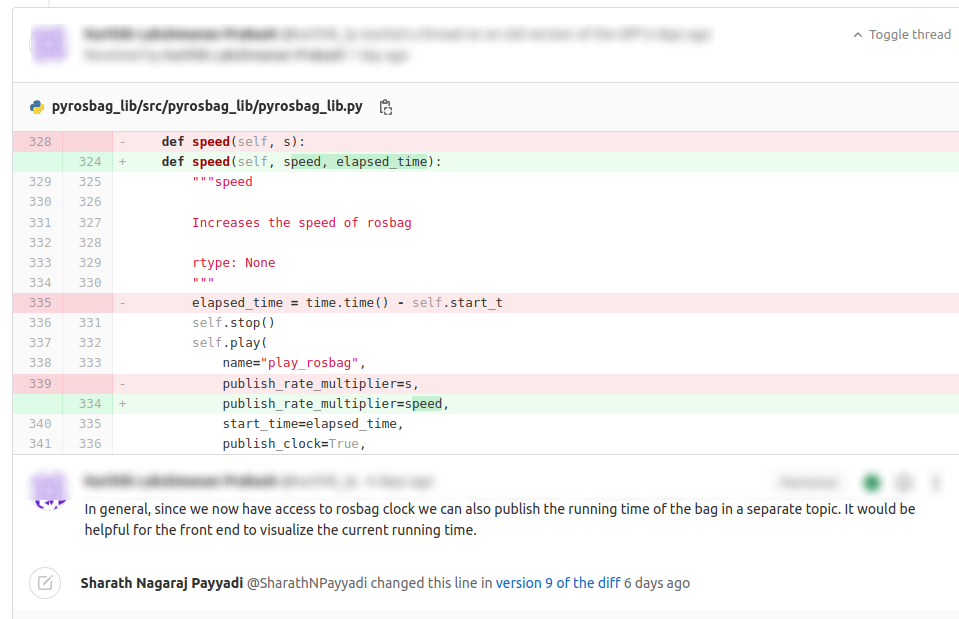
\includegraphics[height=10cm,width=\linewidth]{images/code-review.png}
		\caption{Code review}
	\end{center}
\end{figure}
 
\section{CI/CD}
The third part of verification comes with CI/CD tool. This is tool which enable to integrate our code with companies code. This CI/CD pipeline will be checked once when the merge request is created to the master branch. In this CI/CD tool different jobs have been defined. Some of the jobs are like black, mypy, code\_quality, catkin lint, check suitably for melodic and noetic. For example black will make sure that written python code is universally standard. 

This toll mainly focuses on the improvement of the code quality and versatility of the code. 

\begin{figure}[h]
	\begin{center}
		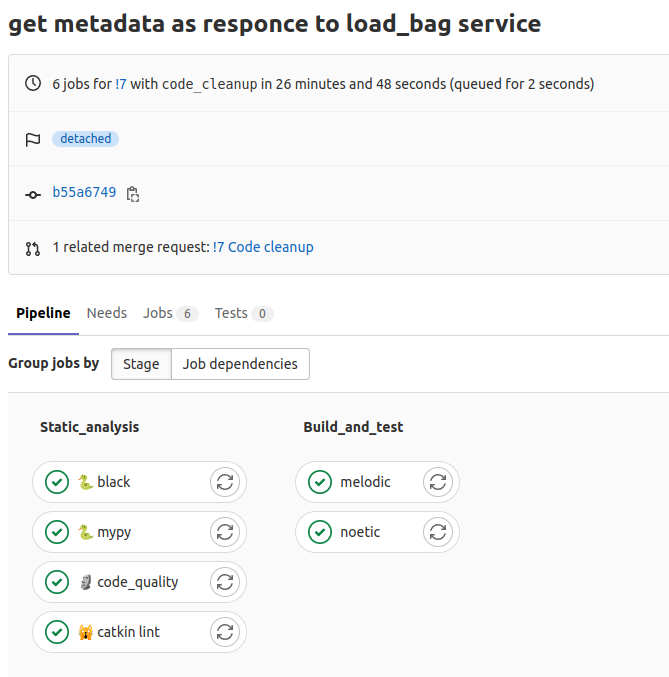
\includegraphics[height=10cm]{images/cicd.png}
		\caption{CI/CD pipelines}
	\end{center}
\end{figure}
\pagebreak
\section{Integration of frontend and backend}
The last part of verification and validation includes the integration of both backend and frontend code. Since the implementation of backend takes place using docker. So we needed to build the image to test the functionality. With the actual implementation we got more reviews. 

This part mainly focuses on the actual working which helps to entangle the future problem